\begin{figure}
	\centering
	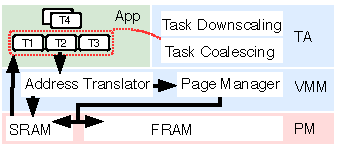
\includegraphics[width=\columnwidth]{figures/system_overview.pdf}
	\caption{\sys top-level view. \sys core innovation are \emph{Adaptive Task Scheduler (TA)} and \emph{Virtual Memory Manager (VMM)}. (PM) stands for Phyical Memory, (App) for applicaiton, and (Tx) for Task.
	\label{fig:system_overview}
\end{figure}
%
\sys is a new programming and execution model for intermittent computing on energy-harvesting devices. \sys addresses the challenges outlined in Section~\ref{sec:background} to make task-based intermittent programs {\em programmable}, {\em efficient} and {\em portable}. \sys accomplishes this goal with a constellation of a new programming model and runtime software system support, that supports dynamically adaptive task-based execution. Fig.~\ref{fig:system_overview} shows an overview of \sys.

\textbf{Programming and Execution Model.}  To use \sys, a programmer must (i) convert a plain C code into tasks by encapsulating the code in a top-level set of functions, (ii) sequence the control-flow between these tasks, and (iii) annotate memory accesses that manipulate global data. The programmer compiles their task-based code, and links to \sys runtime, producing a \sys-enabled binary. The runtime library relies on \sys's novel {\em adaptive task scheduler} to adapt its execution with the energy conditions. The scheduler itself required specialized memory management, which we denote as {\em virtual memory manager}.

\textbf{Adaptive Task Scheduler.} \sys's adaptive task scheduler (ATS) makes \emph{energy-aware} scheduling decisions to group tasks together or split a task. By coalescing tasks \sys amortizes commit and transition costs, and by a task splitting, after repeated failures on a single task, it avoids the task non-termination problem. The scheduler uses only its recent execution history---i.e. it is hardware independent---as a metric to estimate energy availability and eventually to decide on the dynamic task size. Section~\ref{sec:task_adaptation} provides details on the ATS.

\textbf{Virtual Memory Manager.} \sys is able to coalesce tasks \emph{only because of} its virtual memory manager (VMM). the VMM privatizes a group of memory pages demanded by a coalesced task, and limits an application access only to the fast volatile memory. It persists all pages modifications in non-volatile memory on a coalesced task transition. Section~\ref{sec:memory_virtulaization} provides details on the VMM.